\section{Design of beamfs 0.1.26}\label{sec:design}

\subsection{The capsule}\label{sec:capsule}

A \bfs data block is 4\,096 bytes (\cref{fig:capsule}). Its first 3\,824
bytes are the data symbols of sixteen RS(255,239) codewords over
GF($2^8$), interleaved: symbol $i$ of codeword $k$ sits at byte
$16i+k$. Bytes 0 to 3\,807 hold file data; bytes 3\,808 to 3\,823 hold a
checksum and a block self-identifier when the volume is formatted with
the optional \texttt{DATA\_CSUM} and \texttt{DATA\_SELFID} features, and
are otherwise unused. The sixteen parity symbols of codeword $k$ follow,
grouped, at byte $3\,824+16k$. The last sixteen bytes carry a generation
number outside every codeword. A file therefore takes one block per
3\,808 bytes: a 256\,KiB file takes 69 data blocks.

Each codeword corrects up to $t=8$ erroneous symbols, so a block
survives up to 128 erroneous bytes if they are spread. Interleaving
decides what spread means. A burst of up to 128 consecutive bytes in the
3\,824 coded bytes puts at most eight symbols in any codeword; 129 put
nine in one, which is lost. The parity is not interleaved: nine
consecutive bytes inside the 16 parity bytes of one codeword are enough
to lose it. That region is 256 bytes, 6.25\,\% of the block. No result
in this report depends on burst tolerance: the injected upsets are
single bits (\cref{sec:setup}).

\begin{figure}[t]
\centering
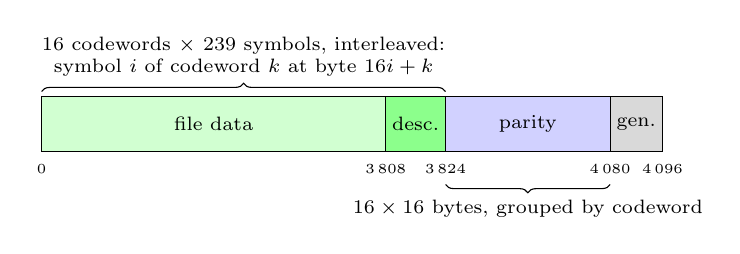
\begin{tikzpicture}[x=0.95mm,y=1mm,font=\scriptsize]
  % not to scale: the coded data is shortened so the small regions read
  \draw[fill=green!18] (0,0) rectangle (46,7);
  \draw[fill=green!45] (46,0) rectangle (54,7);
  \draw[fill=blue!18] (54,0) rectangle (76,7);
  \draw[fill=gray!30] (76,0) rectangle (83,7);
  \node at (23,3.5) {file data};
  \node at (50,3.5) {desc.};
  \node at (65,3.5) {parity};
  \node at (79.5,3.5) {gen.};
  \draw[decorate,decoration={brace,amplitude=3pt}] (0,7.6) -- (54,7.6)
     node[midway,above=2pt,align=center]{16 codewords $\times$ 239 symbols, interleaved:\\symbol $i$ of codeword $k$ at byte $16i+k$};
  \foreach \x/\l in {0/0, 46/3\,808, 54/3\,824, 76/4\,080, 83/4\,096}
     \node[font=\tiny,anchor=north] at (\x,-0.4) {\l};
  \draw[decorate,decoration={brace,amplitude=3pt,mirror}] (54,-4.2) -- (76,-4.2)
     node[midway,below=2pt,align=center]{$16\times16$ bytes, grouped by codeword};
\end{tikzpicture}
\caption{A \bfs data block under \texttt{INCOMPAT\_RS\_INTERLEAVE}, the
layout of every measured volume; byte offsets below, not to scale. The
descriptor (bytes 3\,808 to 3\,823, checksum and self-identifier) is
inside the code and off on the measured volumes; bytes 4\,080 to 4\,095
hold the generation number, outside the code.}
\label{fig:capsule}
\end{figure}

\subsection{Read path}\label{sec:readpath}

Reading a file range, \bfs reads each data block the page overlaps into
a private scratch page, decodes the sixteen codewords there, and copies
the requested bytes out. A 4\,KiB page straddles two 3\,808-byte
payloads, so a sequential read fetches most blocks twice, each time from
the medium. The decoder runs on every read, whatever any checksum says.
If any codeword is beyond correction the read fails with
\texttt{-EIO} and the event is journalled: \bfs refuses rather than
returns bytes it cannot vouch for.

Correction is applied to the copy. In 0.1.26 the read path does not
write the corrected block back. The on-read repair v2 described was
disabled when decoding moved into a private copy; the source states
that re-enabling it needs exclusive access to the block for the whole
read-modify-write. A background scrubber
decodes allocated data blocks at a bounded pace (one block every
100\,ms by default) and writes a corrected block back only if its owner
and its content have not changed in between and the volume is writable.
Errors on the medium are therefore corrected on every read and repaired
by the scrubber, not by the read.

\subsection{Metadata and indirect blocks}\label{sec:indirect-design}

Inodes carry their own RS parity and a CRC over the whole inode;
directory blocks are RS-encoded; the feature bits of every measured
volume read \texttt{incompat}~\featIncompat{} (per-inode RS, indirect
parity, directory RS, full inode CRC, parity-region FEC, interleave) and
\texttt{ro\_compat}~0, which confirms that \texttt{DATA\_CSUM} and
\texttt{DATA\_SELFID} were off.

An indirect block holds 512 raw 64-bit pointers and has no room for its
own code. Its parity lives in a separate region, one slot per indirect
block, by default in Reed-Solomon mode. The slot covers the first 3\,824
bytes, pointers 0 to 477; pointers 478 to 511 are covered by
nothing~\cite{beamfsimpl} (\texttt{known-limitations.md}, 3.38). In
Reed-Solomon mode the verify step decodes a \emph{copy} of the indirect
block, journals what it found and leaves the buffer alone: an earlier
version corrected the live block against stale parity and erased valid
pointers, so a verify no longer writes. A correctable error is thus
journalled and the pointer is read as it stands. Every pointer is then
checked against the data area and the allocation bitmap, and a pointer
outside either fails the lookup with \texttt{-EUCLEAN}. A flipped pointer
that stays inside the data area and lands on an allocated block passes
every check; without \texttt{DATA\_SELFID} nothing detects it. The
project recorded one such case on a direct pointer, 15\,245 wrong bits
returned with no kernel signal (comment in \texttt{file\_inline.c} at
\texttt{\commitBeamfs}). \Cref{sec:indirect} reports what the campaign
did to indirect blocks.
